\documentclass[10pt,a4j,twocolumn]{ltjsarticle}

% 実験V報告書様式
\usepackage{experiments_v}

% ソースコード表示
\usepackage{listings}
% 色
\usepackage{xcolor}
% 数学関連
\usepackage{amsmath, amssymb}
% リスト制御
\usepackage{enumitem}
% newtxフォント
\usepackage{newtxmath, newtxtext}
% 画像
\usepackage{graphicx}
% shaded環境の背景色の定義
\definecolor{shadecolor}{gray}{0.80}
% 枠
\usepackage{ascmac}
\usepackage{tcolorbox}
% url表記
\usepackage{url}
% ハイパーリンク
\usepackage[pdfencoding=auto]{hyperref}
% フォント
\usepackage{layouts/lualatexsets/fonts}
% Tikz関係
\usepackage{tikz}
% 証明などのスタイル
\usepackage{layouts/others/theorem}
% セクションの表示スタイル
%\usepackage{layouts/others/section}
% ベクトル表記
\usepackage{bm}
\def\vector#1{\mathop{\mathbf{#1}}}
% 疑似アルゴリズム
\usepackage{algorithm}
\usepackage{algorithmic}
% 画像・図表等のrefコマンド
\def\thmref#1{Thm. \ref{#1}}
\def\lmmref#1{Lemma. \ref{#1}}
\def\figref#1{図\ref{#1}}
\def\eqref#1{(\ref{#1})式}
\def\tableref#1{表\ref{#1}}

%%% 著者情報 %%%
% 出席番号
\attendancenumber{32}
% 著者
\author{萩原 涼介}
% タイトル
\title{クラスタ数推定に用いる最適な情報量基準の探求}
% 指導教員
\adviser{藤田 一寿}
% 日付
\date{2017年8月4日}

\hypersetup{%
  colorlinks=true,%
  urlcolor=black,%
  linkcolor=black,%
  citecolor=black,%
  linktocpage=true,%
  bookmarks=false,%
  pdftitle={情報工学実験V 報告書},%
  pdfsubject={クラスタ数推定に用いる最適な情報量基準の探求},%
  pdfauthor={Hagihara Ryosuke},%
  pdfkeywords={クラスタリング; 情報量規準; クラスタ数推定; 機械学習}
}

\begin{document}
\maketitle
\section{はじめに}
クラスタリングとはデータを教師なし学習により任意の数のクラスタに分ける手法である.
クラスタリングはデータ解析,データマイニング,パターン認識など様々な分野で用いられる.
多くのクラスタリング手法では,予めクラスタ数を指定しクラスタリングを行う.
しかし,データに対し最適なクラスタ数を指定しなければ,最適なクラスタリング結果を得ることはできない.
その為,クラスタ数を推定することは重要な課題となっている.

既存のクラスタ数推定手法の多くは,情報量規準に基づきクラスタ数の推定を行っている.
情報量規準とは簡単に言えば確率分布とデータの分布の当てはまり具合を表す.
その情報量基準は多くの研究者により様々なものが提案されている.
しかし,どの情報量規準がどのようなデータに対し有効かは分かっていない.
そこで本研究では,クラスタ数推定に用いる情報量規準として最適なものを数値実験を通し明らかにする.
本研究では,クラスタ数推定の手法としてX-meansを用いる.

\section{実験の経過}
4月から6月は機械学習と確率統計の基礎学習およびPythonの勉強を行った.
6月,7月にクラスタリング手法であるK-meansとX-meansの実装を行った.

\section{実験の手法}
\subsection{K-means}
K-means$^{1)}$は,多次元空間上のデータ点集合について,各データが属するクラスタを同定する最もよく使われるクラスタリング手法の一つである.
K-meansは,以下の2つの手順を繰り返すことでクラスタリングを行う.
\begin{enumerate}
  \item 各データ点とデータ点の距離を求め,各データ点を最も近いセントロイドのクラスタに割り当てる.
  \item クラスタに所属するデータの平均を新たなセントロイドとする.
\end{enumerate}

\subsection{X-means}
X-means$^{2)}$は,データ分布が混合等方Gauss分布から生成されたと想定してクラスタ数推定及び
クラスタリングを行う手法である.
K-meansの逐次繰り返しと,BIC$^{3)}$ (Bayesian Information Criterion; ベイズ情報量規準) による
分割停止規準を用いることで,クラスタ数を推定しクラスタリングを実行する.

具体的には以下の手順で行われる.
% \begin{algorithm}
%   \caption{x-means}
%   \label{alg:x-means}
%   \begin{algorithmic}
%     \REQUIRE $n \geq 0 \vee x \neq 0$
%     \ENSURE $y = x^n$
%     \STATE $y \Leftarrow 1$
%     \IF{$n < 0$}
%     \STATE $X \Leftarrow 1 / x$
%     \STATE $N \Leftarrow -n$
%     \ELSE
%     \STATE $X \Leftarrow x$
%     \STATE $N \Leftarrow n$
%     \ENDIF
%     \WHILE{$N \neq 0$}
%     \IF{$N$ is even}
%     \STATE $X \Leftarrow X \times X$
%     \STATE $N \Leftarrow N / 2$
%     \ELSE[$N$ is odd]
%     \STATE $y \Leftarrow y \times X$
%     \STATE $N \Leftarrow N - 1$
%     \ENDIF
%     \ENDWHILE
%   \end{algorithmic}
% \end{algorithm}
\begin{enumerate}
    \item クラスタ数$k$を初期化する (通常は$k=2$) .
    \item K-meansを実行する.
    \item 次の処理を$j=1$から$j=k$まで繰り返す.
    \begin{enumerate}
        \item クラスタ$j$のBIC$_j$を計算する.
        \item クラスタ$j$に所属するデータに対し,クラスタ数2としてK-meansを行う.
        \item クラスタ数2としてクラスタリングした結果に対しBIC'$_j$を計算する.
        \item BIC$_j$とBIC'$_j$を比較し,BIC'$_j$が大きければクラスタ数$k$に1を足す.
    \end{enumerate}
    \item 前の処理で$k$が増加した場合は処理2へ戻る.そうでない場合は終了する.
\end{enumerate}

X-meansで用いるBICは次のように求められる.
$d$次元のデータ${\bm D}=({\bm x_0}, {\bm x_1}, \cdots, {\bm x_d})$を
$K$個のクラスタに分割することを考える.
モデル$M_j$の評価に用いるBICは以下で与えられる.
\begin{align}
  \label{eq:bic}
  \mathrm{BIC}(M_j) = \hat{l}_j(D) - \frac{p_j}{2}\ln R
\end{align}
$p_j$はモデル$M_j$のパラメータ数であり,$R$は$M_j$のデータ数,
$\hat{l}_j(D)$は$p$変量Gauss分布の対数尤度関数である.

等方Gauss分布を考えると分散$\sigma^2$は\eqref{eq:variance}により表される.
\begin{align}
  \label{eq:variance}
  \hat{\sigma}^2 = \frac{1}{R-K}\sum_i\left({\bm x}_i-{\bm \mu}_{(i)}\right)^2
\end{align}
すると,確率は次で表される.
\begin{align}
  \label{eq:gaussian-distribution}
  \hat{P}(x_i) = \frac{R_{(i)}}{R}\frac{1}{\sqrt{2\pi}\hat{\sigma}^d}
    \exp\left(-\frac{1}{2\hat{\sigma}^2}||{\bm x}_i-{\bm \mu}_{(i)}||^2\right)
\end{align}
ここで${\bm \mu}_{i}$は$d$次元の平均ベクトルである.
したがって対数尤度関数は
\begin{align}
  \label{eq:log-likelihood}
  l(D) &= \log \prod_i P(x_i) \\\nonumber
  &= \sum_i \left( \log\frac{1}{\sqrt{2\pi}\sigma^d}-\frac{1}{2\sigma^2}||{\bm x}_i-{\bm \mu}_{(i)}||^2 + \log\frac{R_{(i)}}{R} \right)
\end{align}
となる.
ここでクラスタ$n (1 \leq n \leq K)$のデータ$D_n$に着目する.
クラスタ$n$のデータ数を$R_n$と表記すると,\eqref{eq:log-likelihood}は以下で表される.
\begin{align}
  \begin{split}
    \hat{l}(D_n) &= -\frac{R_n}{2}\log(2\pi) - \frac{R_n \cdot d}{2}\log(\hat{\sigma}^2) -
    \frac{R_n - K}{2}\\ &
    + R_n\log R_n - R_n \log R
  \end{split}
\end{align}

\subsection{実験環境}
実験にはPython3.5を用い,
機械学習のライブラリとしてTensorFlowを用いてアルゴリズムを実装した.

\section{実験結果}
\subsection{K-meansによるクラスタリング}
\figref{img:kmeans-before}のデータをクラスタ数5としてクラスタリングした結果,
\figref{img:kmeans-after}のような結果になった.

\begin{figure}[htbp]
  \begin{center}
    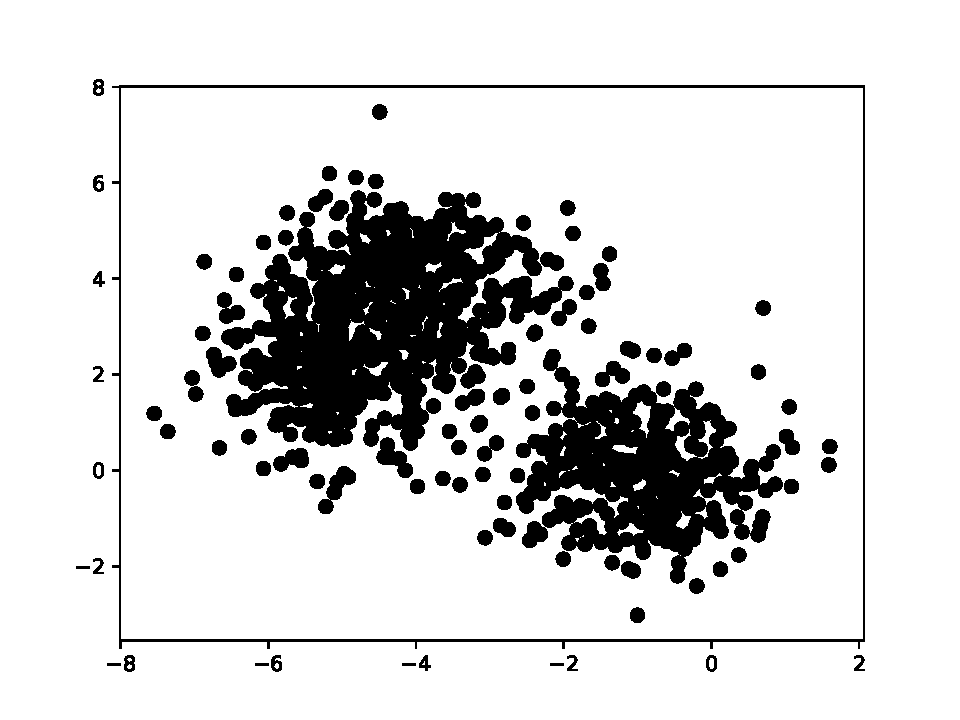
\includegraphics[width=0.8\linewidth]{img/k-means/before.pdf}
    \caption{クラスタリング前のデータ}
    \label{img:kmeans-before}
  \end{center}
\end{figure}
\begin{figure}[htbp]
  \begin{center}
    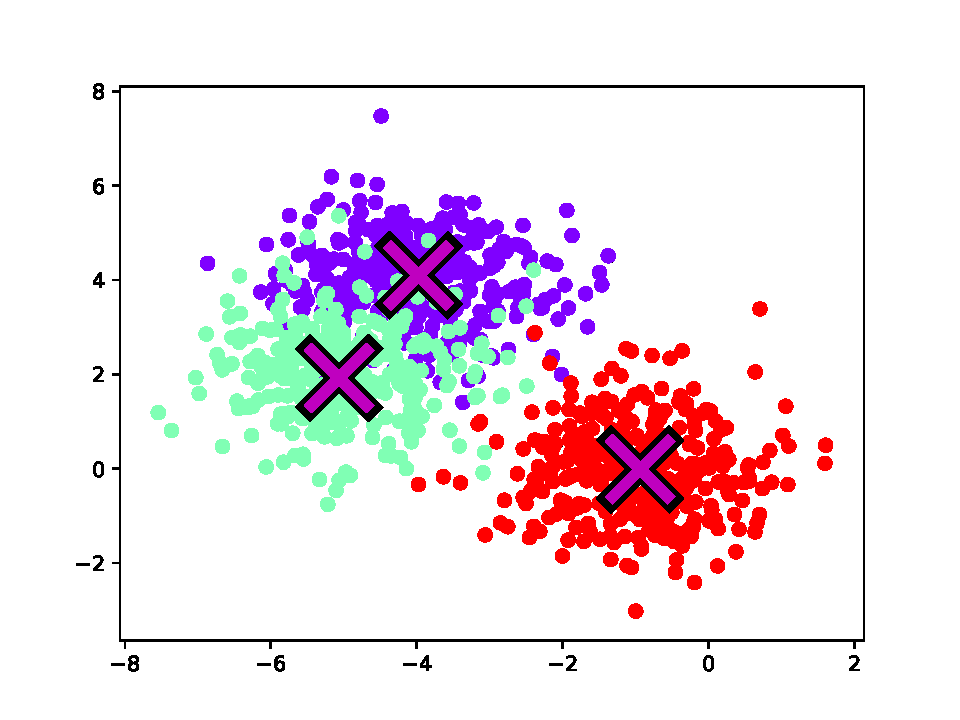
\includegraphics[width=0.8\linewidth]{img/k-means/after.pdf}
    \caption{K-meansによるクラスタリング結果}
    \label{img:kmeans-after}
  \end{center}
\end{figure}

\subsection{X-meansによるクラスタリング}
K-meansと同様に,クラスタ数が5つのデータを生成し,X-meansにより分割した結果,
\figref{img:xmeans-after}のようになった.
図より,クラスタ数を5つとして適切にクラスタリングを行っていることがわかる.

\begin{figure}[htbp]
  \begin{center}
    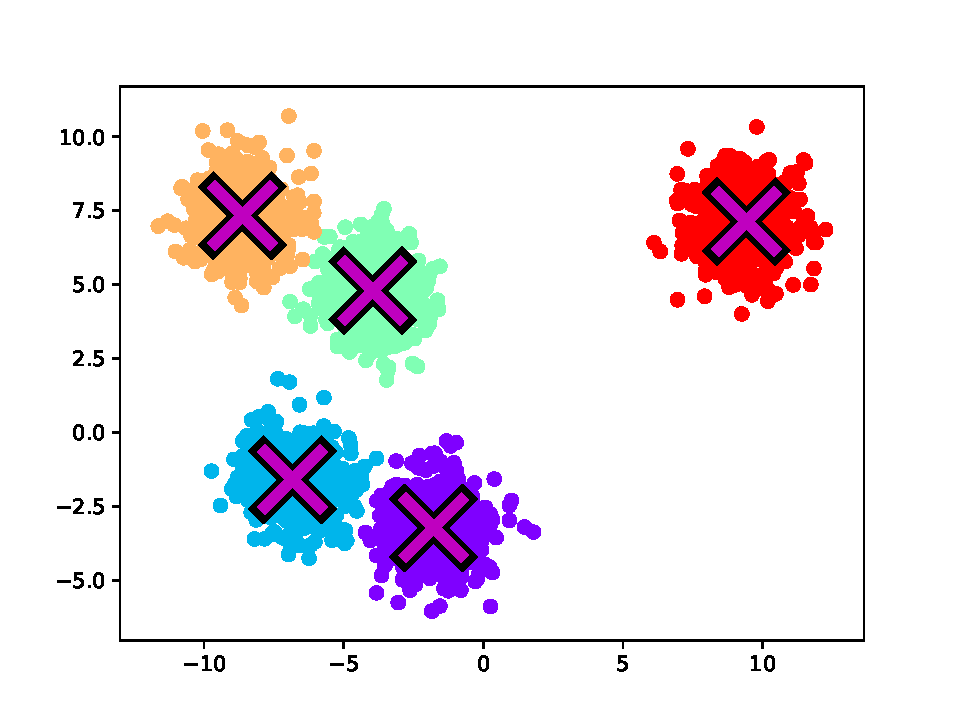
\includegraphics[width=0.8\linewidth]{img/x-means/after.pdf}
    \caption{X-meansによるクラスタリング結果}
    \label{img:xmeans-after}
  \end{center}
\end{figure}

\section{おわりに}
本実験では,機械学習の基礎学習及びK-means, X-meansの実装を行った.
先に示した実験結果より,X-meansは適切にクラスタ数を推定し,
クラスタリングを行うことが確認された.
現在は分割停止規準としてBICを用いているが,
今後様々な情報量規準を用いて実験を行い,最適な情報量規準を明らかにしたい.
クラスタリング精度について検証を行っていきたい.

\section{参考文献}
\begin{enumerate}
\renewcommand{\labelenumi}{\arabic{enumi})}
  \item James MacQueen et al.:
    Some methods for classification and analysis of multivariate observations,
    Proceedings of the fifth Berkeley symposium on mathematical statistics and probability,
    Vol. 1, No. 14, pp. 281--297 (1967).
  \item Dan Pelleg, Andrew W Moore, et al.:
    Xmeans: Extending K-means with Efficient Estimation of the Number of Clusters.,
    ICML, Vol. 1, pp. 727--734 (2000).
  \item Gideon Schwarz et al.:
    Estimating the dimension of a model,
    The annals of statistics, Vol. 6, No.2, pp. 461--464 (1978).
\end{enumerate}
\end{document}
